%%% Compile only with XeLaTeX or LuaLaTeX %%%
% !TeX program = lualatex
\documentclass{beamer}
\usepackage[T1]{fontenc}
\usepackage[orientation = portrait, size = a0]{beamerposter}
\usetheme[blue]{compmat} % also available [red], which is default
\usecolortheme{compmat}
\usepackage{tabularray} %if not available on your machine, compile with Overleaf


\usepackage[utf8]{inputenc}
\usepackage{float}
\usepackage[english]{babel}
\usepackage{tikz-cd}
\usepackage{amsthm}

\usepackage{bbm}
\usepackage{enumitem}
\usepackage{tikz}
\usetikzlibrary{shapes.geometric, positioning, fit}
\usepackage{amsmath}
\usepackage{amsfonts}
\usepackage{amssymb}
\usepackage{mathtools}
\usepackage{graphicx}
\usepackage{rotating}
\usepackage{setspace}
\usepackage{color}
\usepackage{fancyhdr}
\usepackage{ragged2e}
\usepackage{appendix}
\usepackage{tabularx}
\usepackage{multirow}
\usepackage{booktabs}
\usepackage{xfrac}
\usepackage{xcolor}
\usepackage{pgfplots}
\usepackage{url}
\usepackage{emptypage}
\usepackage{wrapfig}
\usepackage{dsfont}
%\usepackage{makecell}
\usepackage{bm}
%\usepackage{csquotes}
\usepackage{quiver}

%new commands


%Operators
\DeclareMathOperator{\CVar}{CVar}
\DeclareMathOperator{\Span}{Span}
\DeclareMathOperator{\fq}{q}
\DeclareMathOperator{\fb}{b}

%shortcuts
\newcommand{\nc}{\newcommand} 
\nc{\cH}{{\mathcal H}}
\nc{\cR}{{\mathcal R}}
\nc{\cA}{{\mathcal A}}
\nc{\cG}{{\mathcal G}}
\nc{\cC}{{\mathcal C}}
\nc{\cD}{{\mathcal D}}
\nc{\cO}{{\mathcal O}}
\nc{\cI}{{\mathcal I}}
\nc{\cB}{{\mathcal B}}
\nc{\cY}{{\mathcal Y}}
\nc{\cK}{{\mathcal K}} 
\nc{\cX}{{\mathcal X}}
\nc{\cS}{{\mathcal S}}
\nc{\cE}{{\mathcal E}}
\nc{\cF}{{\mathcal F}}
\nc{\cZ}{{\mathcal Z}}
\nc{\cQ}{{\mathcal Q}}
\nc{\cN}{{\mathcal N}}
\nc{\cP}{{\mathcal P}}
\nc{\cL}{{\mathcal L}}
\nc{\cM}{{\mathcal M}}
\nc{\cT}{{\mathcal T}}
\nc{\cW}{{\mathcal W}}
\nc{\cU}{{\mathcal U}}
\nc{\cJ}{{\mathcal J}}
\nc{\cV}{{\mathcal V}}
\nc{\bH}{{\mathbb H}}
\nc{\bA}{{\mathbb A}}
\nc{\bG}{{\mathbb G}}
\nc{\bC}{{\mathbb C}}
\nc{\bO}{{\mathbb O}}
\nc{\bI}{{\mathbb I}}
\nc{\bB}{{\mathbb B}}
\nc{\bY}{{\mathbb Y}}
\nc{\bK}{{\mathbb K}} 
\nc{\bX}{{\mathbb X}}
\nc{\bS}{{\mathbb S}}
\nc{\bE}{{\mathbb E}}
\nc{\bF}{{\mathbb F}}
\nc{\bZ}{{\mathbb Z}}
\nc{\bQ}{{\mathbb Q}}
\nc{\bN}{{\mathbb N}}
\nc{\bP}{{\mathbb P}}
\nc{\bL}{{\mathbb L}}
\nc{\bM}{{\mathbb M}}
\nc{\bT}{{\mathbb T}}
\nc{\bW}{{\mathbb W}}
\nc{\bU}{{\mathbb U}}
\nc{\bD}{{\mathbb D}}
\nc{\bJ}{{\mathbb J}}
\nc{\bV}{{\mathbb V}}
\nc{\bR}{{\mathbb R}}

\nc{\boB}{{\mathbf{B}}}
\nc{\boL}{{\mathbf{L}}}
\nc{\boG}{{\mathbf{G}}}


\nc{\tV}{{\Tilde{{V}}}}
\nc{\tI}{{\Tilde{{I}}}}
\nc{\tY}{{\Tilde{{Y}}}}
\nc{\tS}{{\Tilde{{S}}}}

\nc{\fr}{{\rightarrow}}
\nc{\co}{{\nabla}}

\newcommand{\la}{\; \longrightarrow \;}
\nc{\cu}{{\barline{\nabla}}}

\newtheorem{prop}[theorem]{Proposition}
\newtheorem{defi}[theorem]{Definition}
\newtheorem{oss}[theorem]{Observation}
\newtheorem{theo}[theorem]{Theorem}
\newtheorem{cor}[theorem]{Corollary}
\newtheorem{assumption}[theorem]{Assumption}

\usepackage{color}
\definecolor{deepblue}{rgb}{0.3,0.3,0.9}
\definecolor{deepred}{rgb}{0.6,0,0}
\definecolor{deepgreen}{rgb}{0,0.5,0}
% Logos
% if you wish to add a secondary logo. Just think \logoright as \includegraphics
\logoright{[height=5cm]{EC-JRC-logo.png}} 

% if you need to put more logos. Put the name of the file and use & as separator
\morelogos{LOGO-UNIPV.pdf} 

% Title etc
\title{A parallelization algorithm for the Capacity Expansion Problem of an Electrical Grid}

\author{\textbf{Gabor Riccardi}\inst{1}  }

% \samelineand is just an alias for \qquad
\institute{\inst{1}Università degli Studi di Pavia \samelineand
		   \inst{2}Joint Research Centre (JRC)}


\begin{document}
\begin{frame}[fragile, t]
	\begin{columns}[T]
		\begin{column}[c]{0.3\textwidth}
			\begin{block}{Introduction}
				\begin{itemize}
					\item The European electricity system is undergoing significant
					changes motivated by the EU’s ambition to achieve climate
					neutrality.
					\item The European Resource Adequacy Assessment (ERAA), provides an instrument for detecting and measuring adequacy concerns, which are becoming the basis for the implementation of capacity mechanisms.
					\item Given the size of the problem, only reduced Stochastic Models have been considered, using only 3 uncertainty realizations.
					\item Consequently there it is important to develop a more reliable and robust Adequacy Assessment method for large scale electrical grids.
				\end{itemize}

			\end{block}
			\begin{alertblock}{Goal:}
				\textbf{Develop a parallelization algorithm for the Capacity Expansion Problem (CEP) used for the Adequacy Assessment.}
			\end{alertblock}
			\begin{block}{Economic Dispatch (ED)}
				The Economic Dispatch calculates the operation cost of an electrical grid given a scenario \(\omega = (\mathcal{PV}, \mathcal{W}, \mathcal{D})\) comprising of respectively solar power, wind power and loads.
			
				\begin{align}
					\min_{y} \; & q'y_{\omega}                                                                                                                                           \\
					s.t. \;     & \text{(Power Flow Conservation)} \nonumber \\
								& p_{n,g,t,{\omega}} + bd_{n,t,{\omega}} + \sum_{l \in \cL(n)}f_{n,l,t,{\omega}} + ls_{n,t,{\omega}} + \mathcal{PV}_{n,t,{\omega}} + \cW_{n,t,{\omega}} =  \\
								& \quad \quad =  \cD_{n,t,{\omega}} + s_{nt.{\omega}} + bc_{n,t,{\omega}} \nonumber                                                                         \\ & \text{(\textbf{Storage Constraints})} \nonumber \\
								& v_{n,t,{\omega}} = v_{n,t-1,{\omega}} + BCE \cdot bc_{n,t,{\omega}} - BDE \cdot bd_{n,t,{\omega}} + A_{n,t,{\omega}}                                     \\ & \text{(Storage and Balancing Limits)} \nonumber \\
								& (v_{n,t,{\omega}}, bc_{n,t,{\omega}}, bd_{n,t,{\omega}}) \leq (BV, BC, BD)                                                                               \\  &\text{(Generation Capacity)} \nonumber\\
								& p_{n,g,t,{\omega}} \leq p^{\text{max}}_{n,g} + x_{n,g}                                                                                                   \\& \text{(Transmission Capacity)} \nonumber \\
								& L^{\text{min}}_{n, l} \leq f_{n,l,t,{\omega}} \leq L^{\text{max}}_{n, l}                                                                                 \\ 
				\end{align}
			
				Where \(v_{n,t,w}\) is the power stored at bus \(n\) at time \(t\) and \: \( y_{\omega} = (p_{\omega},f_{\omega},ls_{\omega}, s)'\) is the vector containing the power generation, power flows, line shedding and spillage variables. 
			\end{block}
			\begin{block}{Capacity Expansion Problem (CEP)}
				\begin{itemize}
				\item (CEP) is a two stage stochastic program in which first stage determines the capacity expansion \(x_{n,g}\) for each generator \(g \in \cG \)  
				\item The second stage solves the Economic Dispatch. 
				\end{itemize}
				\begin{align*} 
					\min_{x} \; & c'x + \bE_{\omega}\left[\cV(x,\omega)\right] \\  \tag{CEP}
					s.t. \;     & 0 \leq x_{n,g} \leq X_{n,g} & \text{(Generation Capacity Expansion Limits)}
				\end{align*}
				We denote by \(\mathbf{\cV}(x,\omega)\)  the solution to (ED) in function of the expanded capacities \(x\) and the scenario \(\omega\).
			\end{block}
			

		\end{column}%
		\begin{column}[c]{0.3\textwidth}
			
			\begin{block}{Idea}
				
				\begin{minipage}[t]{0.45\textwidth}
					\textbf{Definition:} The \emph{hypergraph} associated to a linear programming problem LP, denoted by \(\mathcal{G} = (\mathcal{N}, \mathcal{E})\), is constructed as follows:
					
				\end{minipage}
				\hfill
				\begin{minipage}[t]{0.45\textwidth}
					
					\begin{figure}
						\begin{tikzpicture}
							% Node style and position setup
							\foreach \i in {1,...,20}
							{
								\pgfmathparse{int(mod(\i-1,5))} % x position
								\edef\x{\pgfmathresult}
								\pgfmathparse{int((\i-1)/5)} % y position
								\edef\y{\pgfmathresult}
								% Draw a dot instead of a labeled circle
								\fill (1.5*\x,-1.5*\y) circle (2pt) coordinate (x\i); % Place a coordinate for referencing
							}
							
							% Hyperedges as polygons
							\draw[thick, fill=blue!50, fill opacity=0.5] (x1) -- (x4) -- (x11) -- cycle;
							\draw[thick, fill=red!50, fill opacity=0.5] (x16) -- (x5) -- (x8) -- (x10) -- cycle;
							\draw[thick, fill=green!50, fill opacity=0.5] (x3) -- (x6) -- (x13) -- cycle;
							\draw[thick, fill=yellow!50, fill opacity=0.5] (x3) -- (x16) -- (x19) -- (x14) -- (x11) -- cycle;
							\draw[thick, fill=violet!50, fill opacity=0.5] (x4) -- (x17) -- (x20) -- (x12) -- (x15) -- cycle;
							
						\end{tikzpicture}
						\caption{Example of LP hypergraph.}
					\end{figure}
				\end{minipage}
				
				\begin{itemize}
					\item The \emph{nodes} \(\mathcal{N}\) of \(\mathcal{G}\) correspond to the variables of the LP.
					\item The \emph{hyperedges} \(\mathcal{E}\) of \(\mathcal{G}\) correspond to each set of variables that appears together in any constraint of the LP.
				\end{itemize}

				\textbf{If a hypergraph features a partition of \(\cN\) with sparse interconnections (few edges) between subsets, we can remove these edges to solve each subset independently}. To do this, we fix a priori the variables in the removed edges. We search for the optimal values for the fixed variables through an iteratively tightened linear program. \\
				\vspace{1cm}
				For instance, in the case of (ED), we leverage the fact that \textbf{the only constraints connecting variables of different days are the storage constraints}:\\
				\begin{minipage}[t]{0.45\textwidth}
					We divide the time horizon into \(K\) intervals, \( \{0,\ldots, t_{1}\},\) \( \ldots,\{t_{K-1}+1,\ldots,t_K\}\) 
					We fix a priori the intermediate storage values \(v_{t_1},\ldots,v_{t_k}\). 
					We refer to as \textbf{(ED-1),...,(ED-K)}, the (ED) problems restricted to each time interval with fixed intermediate and final storage. We denote their optimal value as \(\mathbf{\cV_{k}(x,v_{t_{k}},v_{t_{k+1},\omega})}\).  %this is kind of as saying to the grid, hey you start this storage levels, but must end at this other storage levels
				\end{minipage}
				\hfill
				\begin{minipage}[t]{0.45\textwidth}
					\vspace{0cm}
					\begin{figure}
						\begin{tikzpicture}[plane/.style={draw, thick, fill=blue!20, opacity=0.6}]
							% Define the number of planes
							\newcommand\NumPlanes{4}
							% Define the distance between planes
							\newcommand\DistPlanes{1.5}
							% Define a list of colors
							\def\colors{{"red", "blue", "green", "orange", "purple"}}
						
							% Draw the planes
							\foreach \i in {0,...,\NumPlanes} {
								% Calculate y-shift based on the plane index
								\pgfmathsetmacro\Shift{\i*\DistPlanes}
								% Draw a plane
								\draw[plane] (0+\Shift,0+\Shift) rectangle ++(3,2);
								% Add a label at the top of each plane
								\node at (1.5+\Shift,2.2+\Shift) {ED-\pgfmathparse{int(\i+1)}\pgfmathresult};
							}
						
							% Connect the corners of the planes
							\foreach \i in {1,...,\NumPlanes} {
								\pgfmathsetmacro\j{\i-1}
								\pgfmathsetmacro\Shift{\i*\DistPlanes}
								\pgfmathsetmacro\PrevShift{\j*\DistPlanes}
								% Retrieve color from list
								\pgfmathsetmacro\Color{\colors[\i-1]}
								% Draw connecting segments
								\draw[thick, \Color] (\PrevShift, \PrevShift) -- (\Shift, \Shift);
								\draw[thick, \Color] (3+\PrevShift, 2+\PrevShift) -- (3+\Shift, 2+\Shift);
							}
						\end{tikzpicture}
							
						
						\caption{(ED) hypergraph representation.}
					\end{figure}
				\end{minipage}

			\end{block}

			\begin{block}{Preliminary Observations and Definitions}
				\textbf{Oss 1: }\(\cV(x,\omega) = \min_{\{v_{t_k}\}_{k=1}^K}\sum_{k=0}^{K-1}\cV_{k}(x,v_{t_{k}},v_{t_k+1},\omega)\)  \\ \vspace{1cm}
				Since each function \(\cV_k\) is piecewise linear convex in \(x,v_{t_K},v_{t_{K+1}}\), it can be approximated by a collection of supporting hyperplanes \(\{\pi^w_{i,k}(x,v_{t_k},v_{t_{k+1}})\}\) of each \(\cV_k\). \\ 
				Thus an approximation of (ED) is given by: 
				\begin{align*}
				  \hat{\mathcal{V}}(x,\omega) & = \min_{\{v_{t_k}\}_{k=1}^K} \sum_{k=0}^K \hat{\mathcal{V}}_k(x,v_{t_k},v_{t_{k+1}}) =                           \\
											  & = \min_{\{v_{t_k}\}_{k=1}^K} \sum_{k=0}^K \theta_{k}^{\omega} \tag{ISP}                                          \\
											  & \quad \quad \text{s.t.} \quad \theta_k^{\omega} \geq \pi_{i,k}^{\omega}(x,v_{t_k},v_{t_{k+1}}) \quad \forall i,k
				\end{align*}
				We refer to this problem as the \textbf{Intermediate Storage Problem (ISP)} 
				\\ (I know, very original)
			
				By substituting \(\mathcal{V}(x,\omega)\) with \(\hat{\mathcal{V}}(x,\omega)\) in the definition of (CEP) we obtain the following relaxation:
				  
				\begin{align*}
					\label{CEP-R}
					\min_{x} \; & c'x + \bE_w\left[\hat{\cV}(x,w)\right] \\  \tag{CEP-R}
					s.t. \;     & 0 \leq x_{n,g} \leq X_{n,g}
				\end{align*}
				  After every iteration, the ISP is tightened by adding cuts computed from the duals of the storage constraints of (ED-k) for \(k=1\ldots K \). After a finite number of iterations (CEP-R) becomes exact.  
			\end{block}
		\end{column}
		\begin{column}[c]{0.30\textwidth}
			\begin{block}{Algorithm's Flowchart}
				% https://q.uiver.app/#q=WzAsMTAsWzEsMCwiXFx0ZXh0e0lucHV0fSJdLFsxLDEsIlxcdGV4dHtSLUNFUH0iXSxbMSwyLCJJU1AoXFxvbWVnYSkgXFw7IFxcZm9yYWxsIFxcb21lZ2FcXGluXFxPbWVnYSJdLFswLDMsIlxcdGV4dHtFRC0xfSJdLFsxLDMsIlxcdGV4dHtFRC0yfSJdLFsyLDMsIlxcZG90cyJdLFszLDMsIlxcdGV4dHtFRC1LfSJdLFsxLDQsIlxcdGV4dHtDb21wdXRlIG5ldyBjdXRzIGZvciB9IFZfayBcXDsgXFxmb3JhbGwgayJdLFs0LDQsIlxcYnVsbGV0Il0sWzEsNSwiXFxoYXR7eF5pfSBcXHRleHR7IGlzIENFUC1vcHRpbWFsfSJdLFswLDFdLFsxLDIsIlxcaGF0e3h9XmkiXSxbMiwzLCJ2X3t0XzB9LHZfe3RfMX0iLDFdLFsyLDQsInZfe3RfMX0sdl97dF8yfSIsMV0sWzIsNV0sWzIsNiwidl97dF97ay0xfX0sdl97dF9rfSIsMV0sWzMsN10sWzQsNywiXFx0ZXh0e0R1YWwgbXVsdGlwbGllcnN9IiwxXSxbNSw3XSxbNiw3XSxbNyw4LCJcXHRleHR7aWYgbmV3IGN1dHN9IiwxXSxbOCwxLCJcXHRleHR7QWRkIGN1dHN9IiwxLHsiY3VydmUiOjV9XSxbNyw5XV0=
				\[\begin{tikzcd}[ampersand replacement=\&, scale=0.75, every label/.append style={scale=0.75}, cells={nodes={scale=0.75}}, column sep=small, row sep=small]
					\& {\text{Input}} \\
					\& {\text{R-CEP}} \\
					\& {ISP(\omega) \; \forall \omega\in\Omega} \\
					{\text{ED-1}} \& {\text{ED-2}} \& \dots \& {\text{ED-K}} \\
					\& {\text{Compute new cuts for } V_k \; \forall k} \&\&\& {\text{Add cuts}} \\
					\& \\
					\& {\hat{x^i} \text{ is CEP-optimal}}
					\arrow[from=1-2, to=2-2]
					\arrow["{\hat{x}^i}", from=2-2, to=3-2]
					\arrow["{v_{t_0},v_{t_1}}"{description}, from=3-2, to=4-1]
					\arrow["{v_{t_1},v_{t_2}}"{description}, from=3-2, to=4-2]
					\arrow[from=3-2, to=4-3]
					\arrow["{v_{t_{k-1}},v_{t_k}}"{description}, from=3-2, to=4-4]
					\arrow[from=4-1, to=5-2]
					\arrow["{\text{Dual multipliers}}"{description}, from=4-2, to=5-2]
					\arrow[from=4-3, to=5-2]
					\arrow[from=4-4, to=5-2]
					\arrow["{\text{if new cuts}}"{description}, from=5-2, to=5-5]
					\arrow[ curve={height=40pt}, from=5-5, to=2-2]
					\arrow["{\text{if no new cuts}}"{description},from=5-2, to=7-2]
				\end{tikzcd}\]
			\end{block}
			\begin{block}{Convergence Results}
				\begin{itemize}
					\item Since \((CEP-R) \leq (CEP)\) if a \((CEP-R)\) optimal solution has the same cost for \((CEP)\) then it's also \((CEP)\)-optimal. 
				\end{itemize}
				
				\textbf{Oss 2: } It is sufficient to prove that after a finite number of steps \((i)\) of the algorithm we have:
				\begin{equation}
				\hat{\cV}(\hat x^i,\omega) = \cV(\hat x^i,\omega)  \text{ for all }  \omega \in \Omega
				\end{equation}
				
				
				\textbf{Oss 3: }After a finite number of iterations no new cuts are found for \(\cV_k\).
				
				\begin{proof}

					We observe that the number possible normal vectors defining the cuts are finite because they correspond to dual solutions of (ED-k) and thus are less than the number of basis matrices of (ED-k), which do not depend on the intermediate storage values . 
					
					\begin{minipage}[t]{0.45\textwidth}
						Thus after a finite number of steps we have:\\
						 a new cut:\\ \(\bar c (x,v)= \textcolor{deepblue}{p}'(x,v) + b\) \\
						 and an old cut: \\\(\pi(x,v) = \textcolor{deepblue}{p}'(x,v) + \bar b\)\\
						 Having the same normal vector \(\textcolor{deepblue}{p}\).
						
					\end{minipage}
					\hfill 
					\begin{minipage}[t]{0.45\textwidth}
						\vspace{0cm}
						\begin{tikzpicture}[scale=1]
							% Draw axes
							\draw[->] (-1,0) -- (4,0) node[right] {$x$};
							\draw[->] (0,-1) -- (0,3) node[above] {$y$};
			
							% Define function breakpoints
							\def\xbreak{2}
							\def\ybreak{2}
			
							% Draw piecewise function
							\draw[thick] (0,2.3) -- (\xbreak,\ybreak);
							\draw[thick] (\xbreak,\ybreak) --  (4,3);
			
							% Draw tangent line (touching the curve at one point)
							\draw[thick, red] (0,1.5) -- (4,2.5);
			
							% Mark the touching point
							\filldraw[black] (\xbreak,\ybreak) circle (1pt);
			
							% Draw parallel line slightly beneath the first one
							\draw[thick, green] (0,1) -- (4,2);
			
							\draw (3,3) node {$\cV_k$};
							\draw (1,1.90) node[red] {$\pi$};
							\draw (1,1.41) node[green] {$\bar c$};
			
						\end{tikzpicture}
					
					\end{minipage}	
					
					Since both are supporting hyperplanes it follows that \( b = \bar b\) \\(and therefore \( \bar c\) is not a new cut).
				\end{proof}
				
				Since supporting hyperplanes calculated at \(\hat x_i\) match the value of \(\cV(\hat x_i, \omega)\), if a new cut is redundant then the lower approximation \(\hat \cV\) was already exact at \(\hat x_i\) thus: \\ \vspace{1cm}
				\textbf{Oss 4:}	If after the \(i\)-iteration no new cuts are added for some \(i\) and \(k\) then \(\hat{\cV}_k(\hat x^i, \hat v_{k},\hat v_{k+1}) = \cV_k(\hat x^i, \hat v_{k},\hat v_{k+1}). \) \\ 
				\vspace{1cm}
				Putting together the previous observations we obtain finally:
				
				\begin{prop}
					The algorithm converges after a finite number of iterations and \(\hat x^i\) is an optimal solution for (CEP).
				\end{prop}
				
				
			\end{block}
		\end{column}


			
	\end{columns}

	\textcolor{blue!20}{\rule{\linewidth}{2pt}}

\begin{columns}[T]


	\begin{column}[t]{0.3\textwidth}
		\begin{exampleblock}{Example on small AC-DC grid}
			\begin{minipage}[t]{0.45\textwidth}
			We implemented the algorithm on the following network, consisting of both AC and DC lines, different kinds of storage units, solar, gas and wind power for a time horizon of 5 weeks and time steps of one hour.
			\end{minipage}
			\hfill
			\begin{minipage}[t]{0.45\textwidth}
			\begin{figure}
				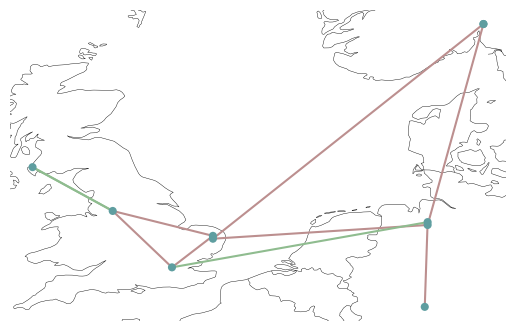
\includegraphics[scale = 0.8]{examplenetwork.png}
				\caption{Network layout.}
			\end{figure}
			\end{minipage}
			\\
			In this instance the algorithm convergence to the optimal solutions in 12 iterations:
			\begin{figure}
				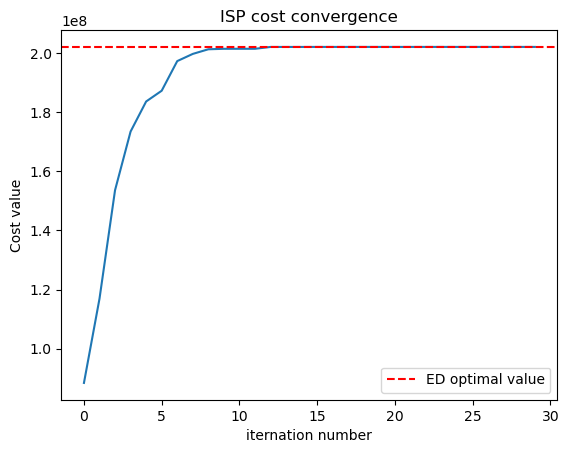
\includegraphics[scale=0.8]{ISPconvergence.png}
				\caption{Objective value of (ISP) for each iteration.}
			\end{figure}
		\end{exampleblock}
	\end{column}
	
		
	
	\begin{column}[t]{0.3\textwidth}
		\begin{alertblock}{Future directions}

			Implement the algorithm in the open source python package Pypsa \\ \vspace{1cm}

			Extend algorithm to general LP: Given the hypergraph \((\cN,\cE)\) associated to LP, we seek a partition of \(\cN\) into disjoint subsets, represented as \(\cN = \sqcup_{i=1}^n\cN_i\). Where any hyperedge connecting \(\cN_i, \cN_j\) with \(i \neq j\) is not connected to any other \(\cN_k\) and has exactly one node in common with one of the two subsets involved.
			\\ \vspace{1cm} Then we could apply the same procedure used for parallelizing ED, splitting the LP in the various \(\cN_i\) and iteratively construct an LP model to get the optimal values of the shared variables.
			\\ The following questions need to be addressed:
			\begin{itemize}
				\item How do we guarantee that (MP) gives solutions which make the LP restricted to each \(\cN_i\) have a feasible solution? \rightarrow \; How to add feasibility cuts?
				\item Is there a way to tell a priori when applying this method is quicker than not parallelizing? \rightarrow \; Consider the size of \(\cN_i\) and number of interconnections between the partition.
			\end {itemize}
			
		\end{alertblock}
	\end{column}%
	\begin{column}[t]{0.3\textwidth}
		\begin{block}{References}
			\begin{thebibliography}{A}
				\bibitem{FirstRef} Daniel Ávila, Anthony Papavasiliou, Mauricio Junca, and Lazaros Exizidis. “Applying High-
	Performance Computing to the European Resource Adequacy Assessment”. In: IEEE Trans-
	actions on Power Systems (2023), pp. 1–13.
				\bibitem{SecondRef d}Daniel Bienstock, Mauro Escobar, Claudio Gentile, and Leo Liberti. “Mathematical Pro-
				gramming formulations for the Alternating Current Optimal Power Flow problem”. In: 4OR
				18.3 (July 2020), pp. 249–292. doi: 10.1007/s10288-020-00455-w.

				\bibitem{ThirdRef}T. Brown, J. Hörsch, and D. Schlachtberger. “PyPSA: Python for Power System Analysis”.
	In: Journal of Open Research Software 6.4 (1 2018).
				\bibitem{ForthRef}Fabian Hofmann. “Linopy: Linear optimization with n-dimensional labeled variables”. In:
				Journal of Open Source Software 8.84 (2023), p. 4823.
	
			\end{thebibliography}
		\end{block}
	\end{column}
\end{columns}





\end{frame}



\end{document}